\documentclass[12pt]{report}
\usepackage{hyperref}
\usepackage[pdftex]{graphicx}
\usepackage[normalem]{ulem}
\usepackage[utf8]{inputenc}
\usepackage[english,frenchb,francais]{babel}
\usepackage[T1]{fontenc}
\usepackage{hyperref}
\usepackage{geometry}
\usepackage{wrapfig}


\begin{document}
\geometry{hmargin=2.5cm,vmargin=1.5cm}
  \begin{titlepage}
    \centering
        \vfill
        {\rule{\linewidth}{.5pt}
        \huge
            Optimisation par algorithme génétique\\
          \large
            Influence du paramétrage\\
          \rule{\linewidth}{.5pt}
            \vskip2cm
            Swan Launay - Gabriel Vaubaillon\\
        }
        \vfill
        
\includegraphics[height=1.7cm]{logo/polytech.jpg}
        \hfill
        
\includegraphics[height=1.7cm]{logo/usmb.png}
  \end{titlepage}
  \chapter{Préambule}
    \section{Remerciements}
      Ce rapport représente l'aboutissement du projet de 40 heures qui s'est déroulé entre octobre 2018 et avril 2019. Nous tenons tout d'abord à remercier Gilles Fraisse pour son soutien, sa pédagogie, mais aussi pour le temps qu'il a passé à nous accompagner.

      Nous tenons aussi à remercier l'Université Savoie Mont Blanc (USMB) pour la mise à disposition des documents nécessaires à la réalisation de ce projet par le biais de la bibliothèque universitaire.

      Nous remercions enfin Polytech Annecy - Chambéry pour nous avoir permis d'effectuer ce projet sur notre temps de travail universitaire et plus globalement pour nous avoir proposé un travail de ce type.

    \section{Résumé}
      L'optimisation par algorithme génétique permet d'obtenir de bonnes approximations de résolutions pour différents problèmes (avec un ou plusieurs objectifs). De façon générale, les algorithmes génétiques sont construits de telle façon à ce que l'on puisse faire varier certains paramètres. C'est ces mêmes paramètres qui vont déterminer la qualité et la fiabilité du résultat, mais aussi qui vont faire varier de façon plus ou moins significative le temps de résolution. Il s'agit alors de trouver un juste milieu entre le temps résolution et la fiabilité du résultat.

  \chapter{Introduction}
    Selon la \emph{Théorie de l'évolution} \cite{darwin} de Charles Darwin, l'évolution des espèces est issue de mutations aléatoires qui surviennent lors de la conception d'une nouvelle génération d'individus. Si cette mutation permet à l'individus d'être plus adapté à son milieu de vie, alors il aura plus de chance d'atteindre l'age adulte et d'engendrer une nouvelle génération.
    Les algorithmes génétiques sont une application directe du darwinisme à l'informatique.\\
    De nos jours, ces algorithmes permettent de résoudre des problèmes d'optimisation, c'est à dire de maximiser ou minimiser numériquement une ou plusieurs fonctions.
    La branche des mathématiques qu'est l'optimisation est un élément central dans le monde de l'ingéniérie ou on cherche dans de très nombreux cas à


  \tableofcontents

  \chapter{Optimisation à objectif unique}
    \section{Algorithme}
      \subsection{Principe}
        \begin{wrapfigure}{r}{6cm}
          \centering
          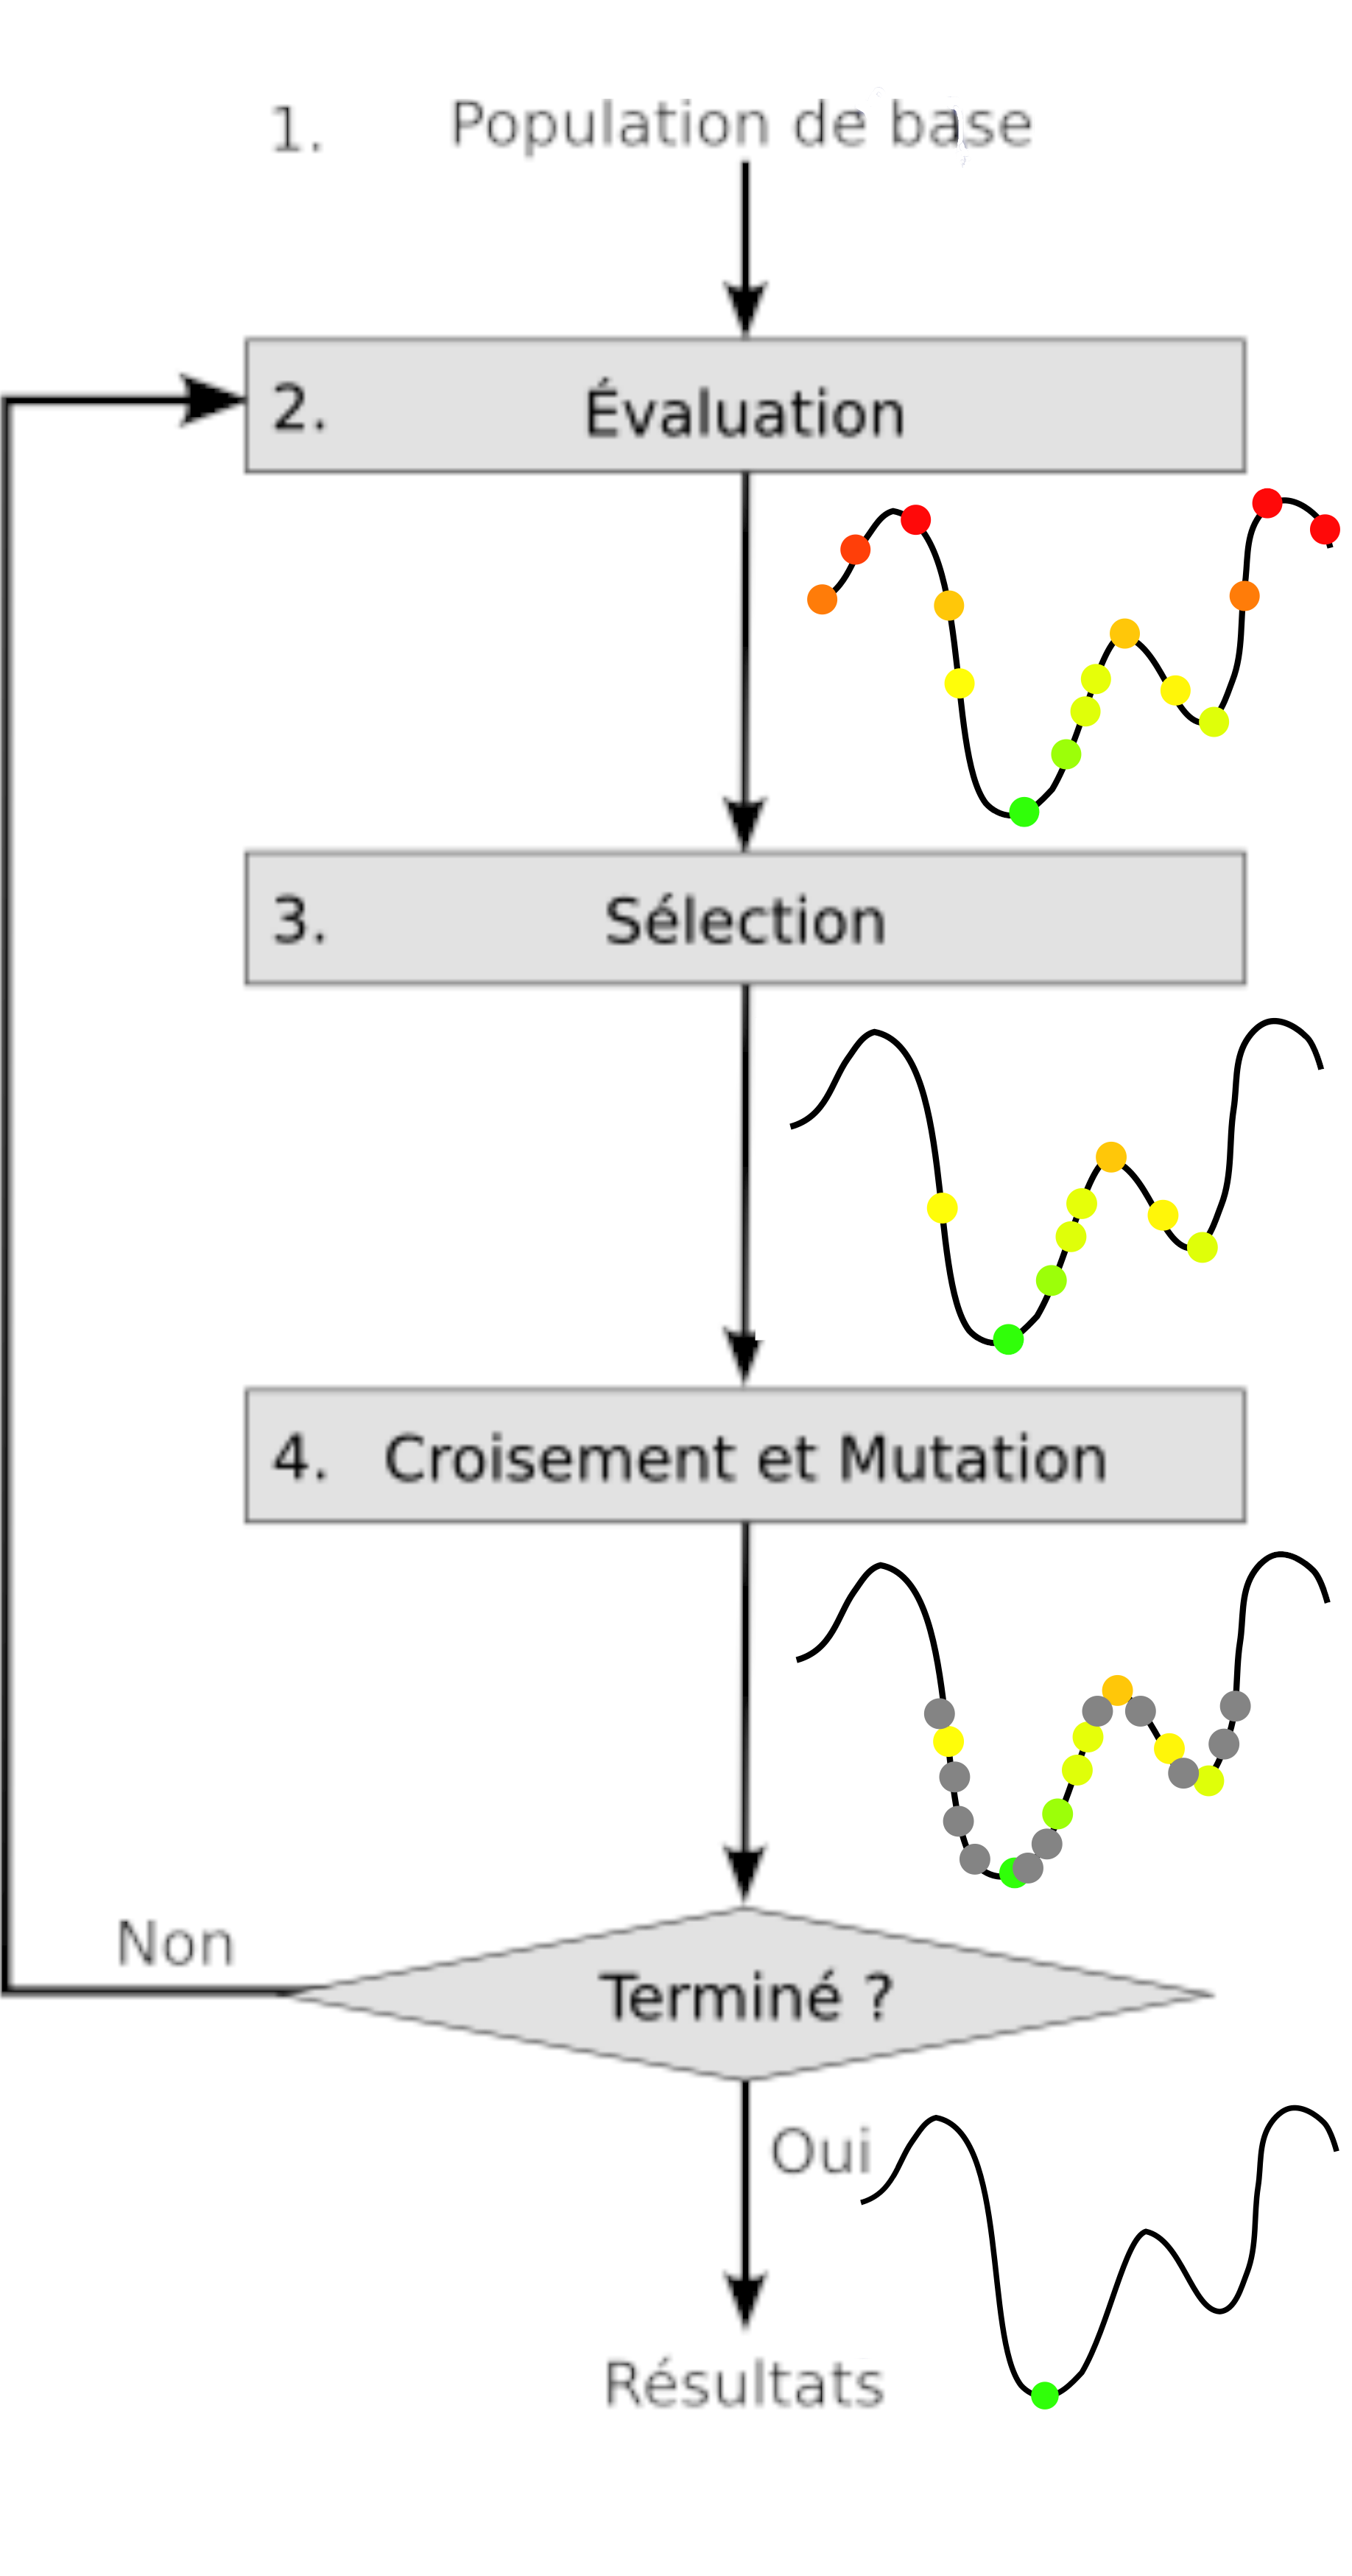
\includegraphics[width=5cm]{img/schema_algo_single.png}
          \caption{Fonctionnement}
        \end{wrapfigure}
        Hormis quelques variations dans leur conception, les algorithmes génétiques on pratiquement tous le même principe de fonctionnement.
        Le logigramme ci-joint illustre le fonctionnement de base de l'algorithme.
        Tout d'abord on génère de façon aléatoire une population de base qui servira d'initialisation de notre algorithme.
        Chaque individus de cette population est alors évalué, on lui attribut donc une valeur qui va déterminer sa position par rapport à la solution optimale recherchée.
        Une selection est alors effectuée en gardant les meilleurs résultats, mais aussi en en gardant un certain poucentage de de valeurs considérée comme de moyenne/faible qualité. Cette dernière opération permet à l'algorithme de ne pas ... dans un extremum local.
        A partir de cette séléction, l'algorithme va ensuite procéder à deux étapes : \\
        Le croisement (Crossover) :
        Il consiste à partager (croiser) les particulartiés de deux individus parents pour engendrer une petite population d'individus conservant ces mêmes particularités. A noter qu'il existe plusieurs méthodes de croisement (un point / deux points)... .
        On retrouve cette opération en biologie sous le nom de "brassage génétique".
        (Principe d'héridité de la théorie de Darwin)
        \begin{figure}
          \centering
          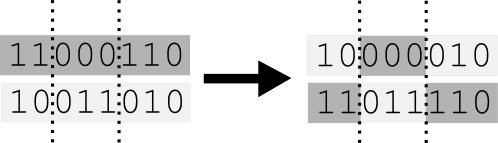
\includegraphics{img/crossover.png}
          \caption{Crossover}
        \end{figure}
        \\
        La mutation :
        Contrairement au croisement qui conserve les particularités des individus au cours des générations, la mutation altère certains individus de manière aléatoire. Cette oprération complète l'opération de séléction précédement évoquée afin d'éviter de tomber dans un extremum local.
        (Principe de variation de la théorie de Darwin)



    \section{Optimisation unidimensionnelle / multidimensionnelle}.

    \section{Influence du paramétrage }



  \chapter{Optimisation à objectifs multiples}
    \section{Algorithme - NSGAII}
    L'algorithmes d'optimisation NSGAII (Non dominated sorting genetic algorithm) est un algorithme connu et utilisé à l'échelle mondiale.
    + Multi obj
      \subsection{Principe}
      + Diff avec algo standard : celui la est élitiste

    \section{Optimisation multidimensionnelle / unidimensionnelle}
    \section{Influence du paramétrage}
    \section{NSGA III}


  \chapter{Conclusion}
   + Il existe d'autre algo utilisés : http://www.laas.fr/files/MOGISA/sem_Alain-Berro.pdf p.31
  \appendix

  \chapter{Bibliographie}
  \nocite{*} %On affiche toute la Bibliographie
  \bibliographystyle{plain}
  \bibliography{biblio}

  \chapter{Annexes}
    \subsection{Programme}
      \paragraph{}
      L'ensemble des programmes qui ont été utilisé pour réaliser ce projet sont mis à disposition sur notre page GitHub : \\\\
      \url{https://github.com/Akashita/TPE-NSGAII}

      \paragraph{}
      Ce travail est soumis à la license \emph{GNU General Public License v3.0}\\ %\emph dit à latex que cette partie est importante
      Pour plus de détails veuillez vous référer au site suivant : \\\\
      \url{https://www.gnu.org/licenses/gpl-3.0.en.html}

    \subsection{Figures}






\end{document}
